\subsection{Perfect Sets and the Cantor Set}

\begin{theorem} \label{thm:nonempty-perfect-subset-rk-uncountable} \hlt{Perfect Sets Are Uncountable}\\
Every nonempty perfect subset of $\R^k$ is uncountable.
\begin{proof}
Assume $P=\{\mathbf{x}_1,\mathbf{x}_2,\ldots\}$. Choose a neighborhood $V_1$ with $V_1\cap P\neq\emptyset$.\\
Inductively, since $P\cap V_n$ contains infinitely many points by Theorem \ref{thm:limit-point-neighborhoods-infinitely-many}, choose $\mathbf{y}_n\in P\cap V_n$ with $\mathbf{y}_n\neq\mathbf{x}_n$ and then a neighborhood $V_{n+1}$ of $\mathbf{y}_n$ such that $\overline{V}_{n+1}\subseteq V_n$ and $\mathbf{x}_n\notin\overline{V}_{n+1}$.\\
Put $K_n\defeq\overline{V}_n\cap P$. Then $K_n$ is nonempty, compact, and $K_{n+1}\subseteq K_n$. By Corollary \ref{cor:nested-nonempty-compact-intersection}, choose $\mathbf{z}\in\bigcap\limits_{n=1}^{\infty}K_n$. For each $n$, $\mathbf{z}\in K_{n+1}$ but $\mathbf{x}_n\notin K_{n+1}$, so $\mathbf{z}\neq\mathbf{x}_n$ for all $n$, contradicting the enumeration.\\
\hlt{Structural Commentary}: Nested compact sets dodge the list.\\
\hlt{Key Insight}: Perfectness gives new points; compactness keeps one.
\end{proof}
\end{theorem}

\begin{figure}[H]
  \centering
  \begin{tikzpicture}[
  every node/.style={font=\small},
  axis/.style={gray!65, line width=0.55pt},
  interval/.style={blue!70!black, line width=1.35pt},
  smallinterval/.style={orange!80!black, line width=1.45pt},
  guide/.style={gray!55, dashed, line width=0.45pt},
  point/.style={circle, fill=black, inner sep=1.45pt}
]
  \draw[axis] (-0.25,0) -- (7.25,0);

  \coordinate (iOneL) at (0.45,0);
  \coordinate (iOneR) at (6.85,0);
  \coordinate (xone) at (2.45,0);
  \coordinate (iTwoL) at (4.35,0);
  \coordinate (ytwo) at (5.05,0);
  \coordinate (iTwoR) at (5.85,0);

  \draw[interval] ($(iOneL)+(0,0.62)$) -- ($(iOneR)+(0,0.62)$);
  \draw[interval] ($(iOneL)+(0,0.34)$) -- ($(iOneL)+(0,0.90)$);
  \draw[interval] ($(iOneR)+(0,0.34)$) -- ($(iOneR)+(0,0.90)$);
  \node[blue!70!black, above] at (3.65,0.92) {$I_1$};

  \draw[smallinterval] ($(iTwoL)+(0,-0.50)$) -- ($(iTwoR)+(0,-0.50)$);
  \draw[smallinterval] ($(iTwoL)+(0,-0.76)$) -- ($(iTwoL)+(0,-0.24)$);
  \draw[smallinterval] ($(iTwoR)+(0,-0.76)$) -- ($(iTwoR)+(0,-0.24)$);
  \node[orange!80!black, below] at ($(ytwo)+(0,-0.78)$) {$I_2$};

  \draw[guide] (iTwoL) -- ($(iTwoL)+(0,-0.50)$);
  \draw[guide] (iTwoR) -- ($(iTwoR)+(0,-0.50)$);

  \node[point] at (xone) {};
  \node[below] at (xone) {$x_1$};

  \node[point] at (ytwo) {};
  \node[above] at (ytwo) {$y_2\in P$};

  \node[gray!65] at (3.40,-0.50) {$x_1\notin I_2$};
\end{tikzpicture}

  \caption{Choose $y_2\in P\cap I_1$ with $y_2\neq x_1$, then take a smaller interval $I_2\subseteq I_1$ around $y_2$ that avoids $x_1$.}
  \label{fig:perfect-set-nested-interval-avoidance}
\end{figure}

\begin{corollary} \label{cor:closed-intervals-and-reals-uncountable} \hlt{Intervals and the Real Line Are Uncountable}\\
Every interval $[a,b]\subseteq\R$ with $a<b$ is uncountable. In particular, $\R$ is uncountable.
\begin{proof}
The interval $I\defeq[a,b]$ is a nonempty $1$-cell, hence compact by Theorem \ref{thm:k-cells-compact} and closed by Theorem \ref{thm:compact-subsets-of-metric-spaces-closed}. For every $x\in I$ and $\varepsilon>0$, $I\cap \bigl(B_{\varepsilon}(x)\setminus\{x\}\bigr)\neq\emptyset$, so $I$ is perfect. Theorem \ref{thm:nonempty-perfect-subset-rk-uncountable} gives that $I$ is uncountable. If $\R$ were countable, then $I\subseteq\R$ would be countable, a contradiction.\\
\hlt{Structural Commentary}: Closed intervals are perfect compact sets.\\
\hlt{Key Insight}: One closed interval already forces $\R$ to be uncountable.
\end{proof}
\end{corollary}

\begin{figure}[H]
  \centering
  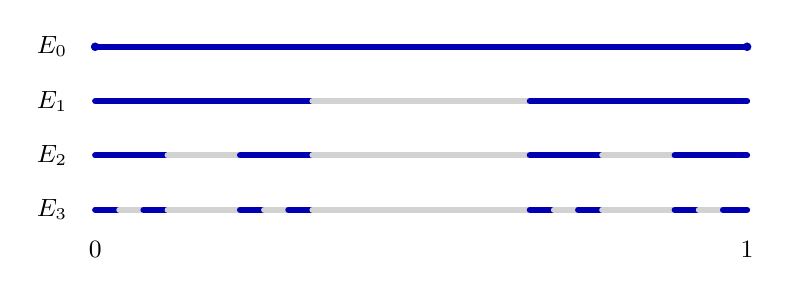
\begin{tikzpicture}[
  every node/.style={font=\small},
  stage/.style={blue!70!black, line width=2.2pt, line cap=round},
  gap/.style={gray!35, line width=2.2pt, line cap=round},
  endpoint/.style={circle, fill=blue!70!black, inner sep=1.1pt},
  scale=0.92
]
  \node[anchor=east] at (-0.25,0) {$E_0$};
  \draw[stage] (0,0) -- (9,0);

  \node[anchor=east] at (-0.25,-0.75) {$E_1$};
  \draw[stage] (0,-0.75) -- (3,-0.75);
  \draw[gap] (3,-0.75) -- (6,-0.75);
  \draw[stage] (6,-0.75) -- (9,-0.75);

  \node[anchor=east] at (-0.25,-1.5) {$E_2$};
  \draw[stage] (0,-1.5) -- (1,-1.5);
  \draw[gap] (1,-1.5) -- (2,-1.5);
  \draw[stage] (2,-1.5) -- (3,-1.5);
  \draw[gap] (3,-1.5) -- (6,-1.5);
  \draw[stage] (6,-1.5) -- (7,-1.5);
  \draw[gap] (7,-1.5) -- (8,-1.5);
  \draw[stage] (8,-1.5) -- (9,-1.5);

  \node[anchor=east] at (-0.25,-2.25) {$E_3$};
  \draw[stage] (0,-2.25) -- (1/3,-2.25);
  \draw[gap] (1/3,-2.25) -- (2/3,-2.25);
  \draw[stage] (2/3,-2.25) -- (1,-2.25);
  \draw[gap] (1,-2.25) -- (2,-2.25);
  \draw[stage] (2,-2.25) -- (7/3,-2.25);
  \draw[gap] (7/3,-2.25) -- (8/3,-2.25);
  \draw[stage] (8/3,-2.25) -- (3,-2.25);
  \draw[gap] (3,-2.25) -- (6,-2.25);
  \draw[stage] (6,-2.25) -- (19/3,-2.25);
  \draw[gap] (19/3,-2.25) -- (20/3,-2.25);
  \draw[stage] (20/3,-2.25) -- (7,-2.25);
  \draw[gap] (7,-2.25) -- (8,-2.25);
  \draw[stage] (8,-2.25) -- (25/3,-2.25);
  \draw[gap] (25/3,-2.25) -- (26/3,-2.25);
  \draw[stage] (26/3,-2.25) -- (9,-2.25);

  \foreach \x in {0,9} {
    \node[endpoint] at (\x,0) {};
  }
  \node[below] at (0,-2.55) {$0$};
  \node[below] at (9,-2.55) {$1$};
\end{tikzpicture}

  \caption{The first stages $E_0,E_1,E_2,E_3$ in the Cantor-set construction.}
  \label{fig:cantor-set-first-stages}
\end{figure}

\begin{example} \label{ex:cantor-set} \hlt{The Cantor Set}\\
Let $E_0=[0,1]$. Remove the open middle third $(1/3,2/3)$ and call the remaining set $E_1$. Continue by removing the open middle third from each interval component, so
\begin{align}
E_1&=[0,1/3]\cup[2/3,1], \nonumber\\
E_2&=[0,1/9]\cup[2/9,3/9]\cup[6/9,7/9]\cup[8/9,1]. \nonumber
\end{align}
Then $E_n$ is a union of $2^n$ compact intervals of length $3^{-n}$ and $E_1\supseteq E_2\supseteq E_3\supseteq\cdots$.\\
The \hlt{Cantor set} is $P\defeq\bigcap\limits_{n=1}^{\infty}E_n$. By Corollary \ref{cor:nested-nonempty-compact-intersection}, $P\neq\emptyset$. Since each $E_n$ is closed and $P\subseteq E_1$, $P$ is a closed subset of the compact set $E_1$, hence compact.\\
If $J\subseteq[0,1]$ is nonempty open interval, for some $m\in\N$ and $k\geq0$, $R_{m,k}\defeq\left(\frac{3k+1}{3^m},\frac{3k+2}{3^m}\right)\subseteq J$ and $R_{m,k}\cap P=\emptyset$.\\
Thus $P$ contains no nontrivial interval. Finally, let $x\in P$ and let $U$ be an interval neighborhood of $x$. If $I_n(x)$ is the component of $E_n$ containing $x$, choose $n$ with $I_n(x)\subseteq U$. An endpoint $y\neq x$ of $I_n(x)$ lies in $P$, so $U\cap(P\setminus\{x\})\neq\emptyset$. Hence $P$ is perfect.\\
\hlt{Structural Commentary}: The Cantor set is built by nested compact deletion, not by listing points.\\
\hlt{Key Insight}: It is compact and perfect, but contains no interval.
\end{example}
